\documentclass[12pt,leqno]{book}
\usepackage{amsmath,amssymb,amsfonts} % Typical maths resource packages
\usepackage{graphics}                 % Packages to allow inclusion of graphics
\usepackage{color}                    % For creating coloured text and background
\usepackage{hyperref}                 % For creating hyperlinks in cross references
\usepackage{url}

% hangul package
\usepackage[hangul,nonfrench]{dhucs}  % For creating hangul package

\parindent 1cm
\parskip 0.2cm
\topmargin 0.2cm
\oddsidemargin 1cm
\evensidemargin 0.5cm
\textwidth 15cm
\textheight 21cm
\newtheorem{theorem}{Theorem}[section]
\newtheorem{proposition}[theorem]{Proposition}
\newtheorem{corollary}[theorem]{Corollary}
\newtheorem{lemma}[theorem]{Lemma}
\newtheorem{remark}[theorem]{Remark}
\newtheorem{definition}[theorem]{Definition}

\def\R{\mathbb{ R}}
\def\S{\mathbb{ S}}
\def\I{\mathbb{ I}}
\makeindex

\title{
Visual Computing : Mixed-Augmented Reality\\
Computer Vision, Graphics and Geometry
}

\author{
Edited by\\
Woonhyuk Baek\\
{\small\em \copyright \  Draft date \today }
}

\date{ }
\begin{document}
\maketitle
 \addcontentsline{toc}{chapter}{Contents}
\pagenumbering{roman}
\tableofcontents

%\listoffigures
%\listoftables

\chapter*{Preface}\normalsize
  \addcontentsline{toc}{chapter}{Preface}
\pagestyle{plain}
Visual Computing\cite{tracking1999}

\pagestyle{headings}
\pagenumbering{arabic}

%chapter1
%Geometry.tex
\chapter{Geometry}\label{ch:geometry}
\begin{center}
{\small\em geometry descriptions...}
\end{center}

\section{Processing Models}
\begin{figure}[!h]
\centering
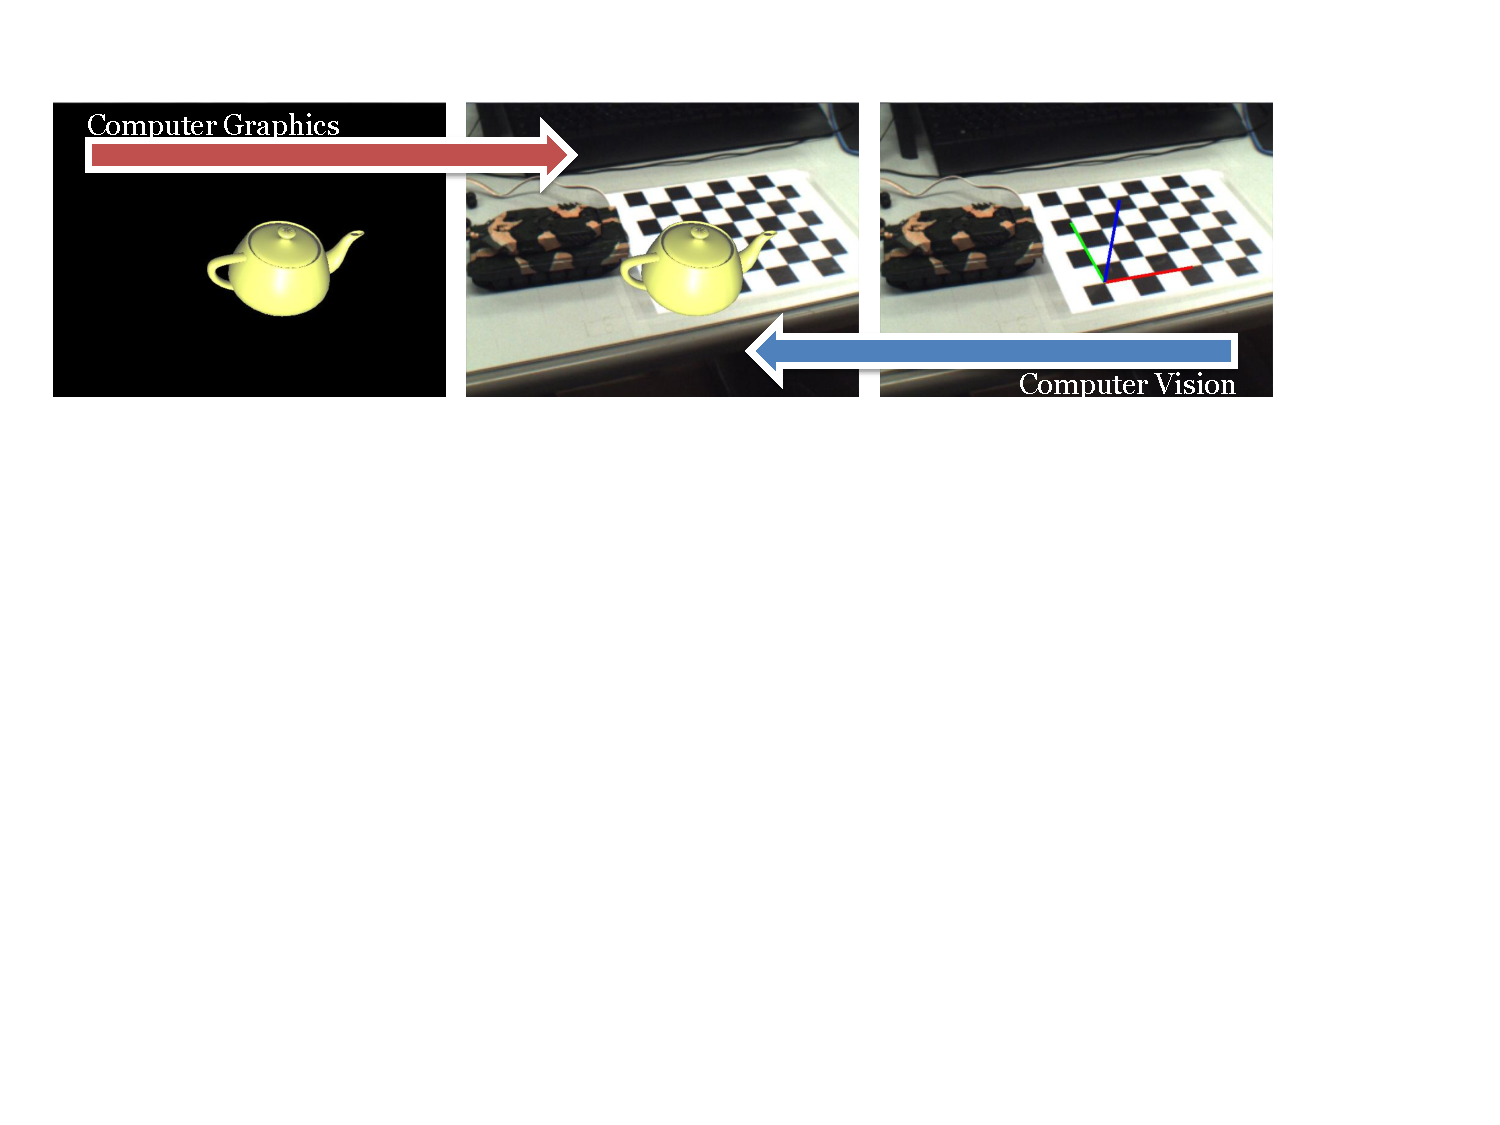
\includegraphics[width=6in]{images/processingmodel.pdf}
\caption{Processing Model using Computer Graphics and Computer Vision for Visual Computing}
\label{fig:processingmodel}
\end{figure}

\section{Camera Models}
A camera is a mapping between the 3D world (object space) and a 2D image\cite{CV_book_multiple_2000_Hartley}.

\begin{figure}[!h]
\centering
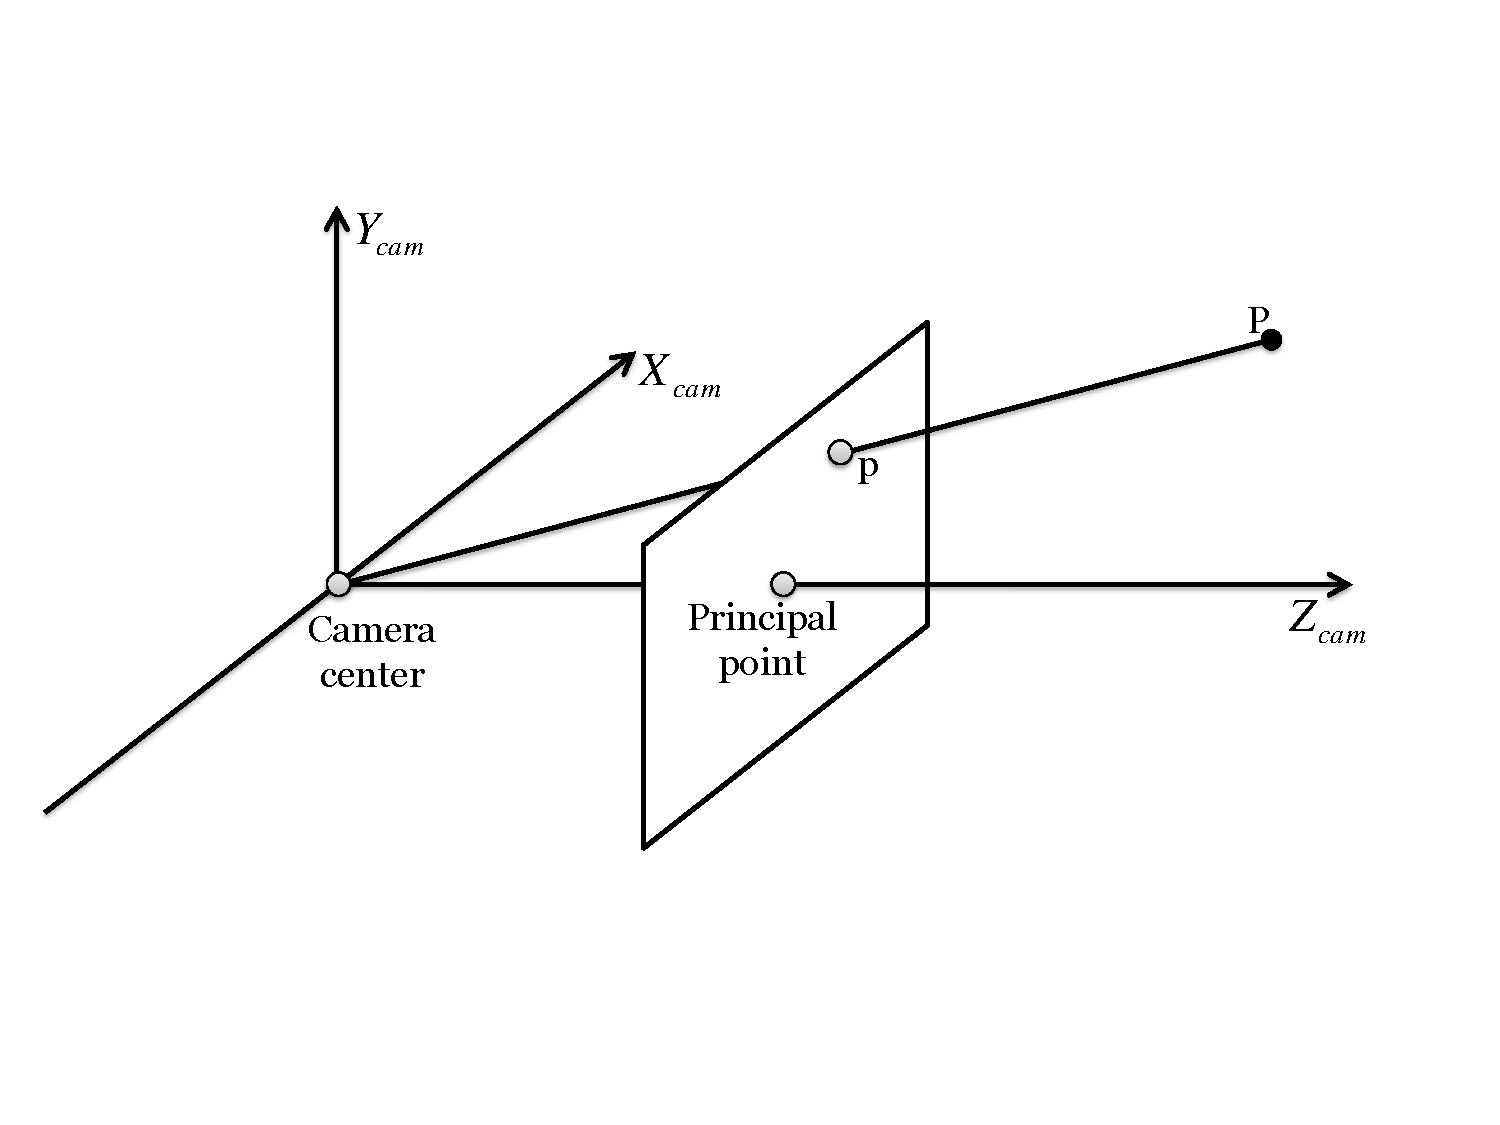
\includegraphics[width=2.5in]{images/cameramodel1.pdf}
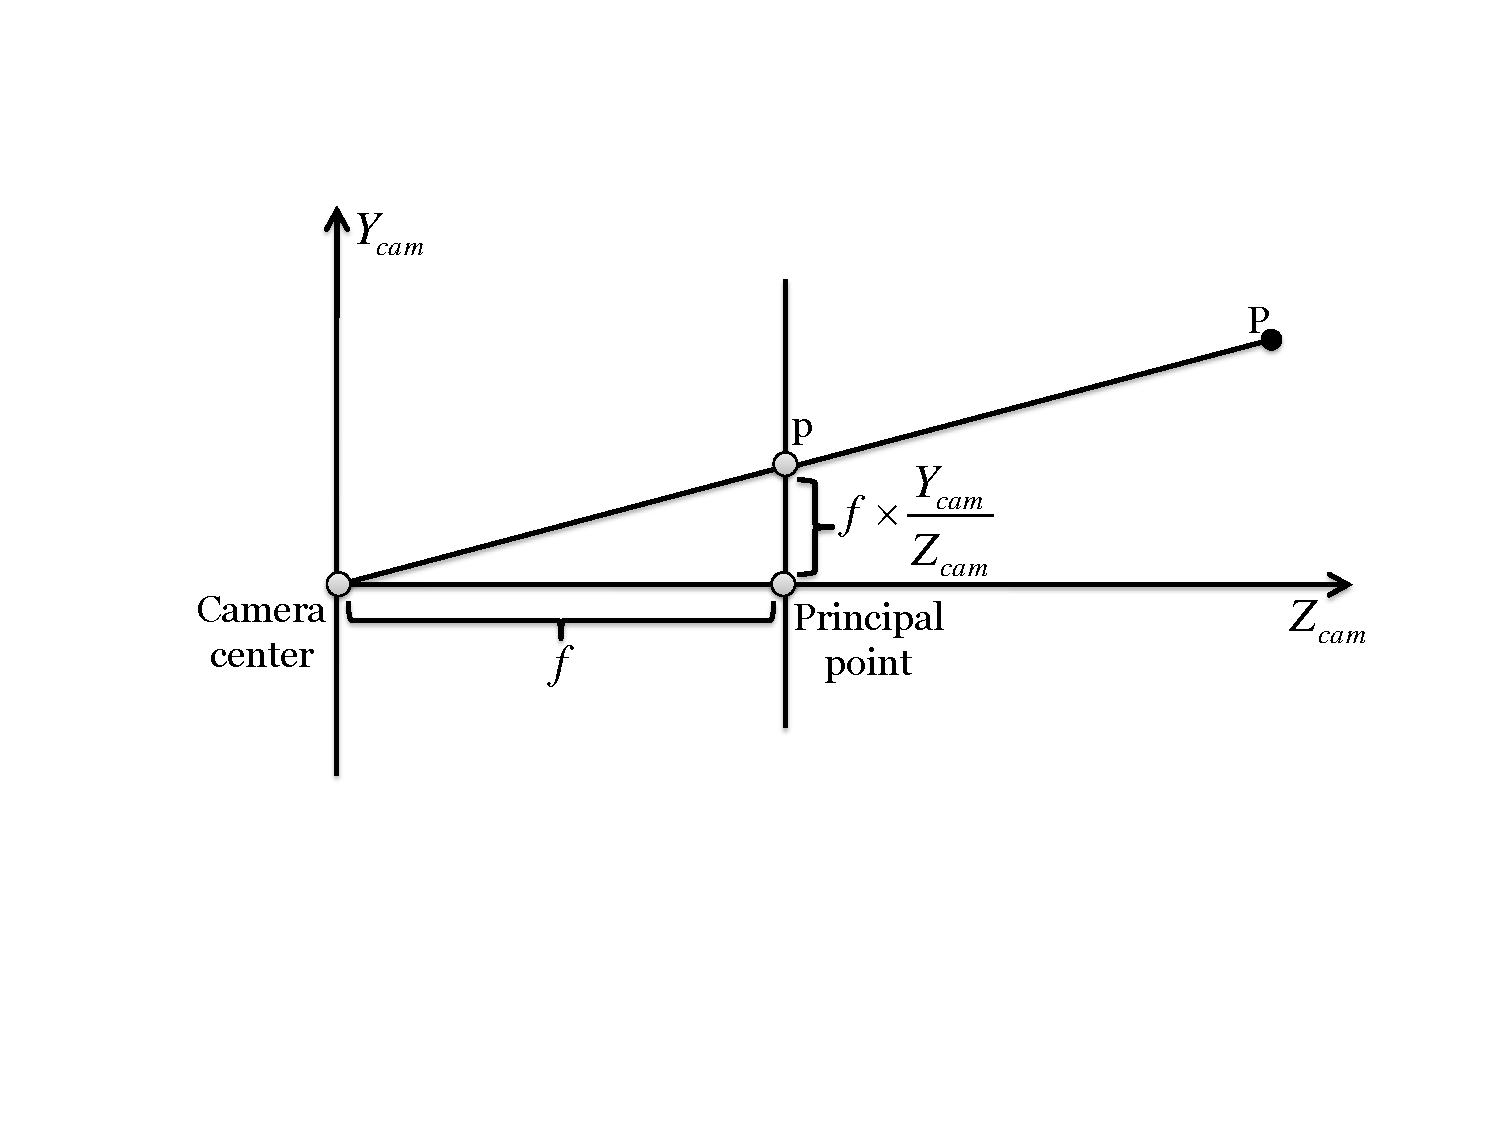
\includegraphics[width=2.2in]{images/cameramodel2.pdf}
\caption{pinhole camera geometry}
\label{fig:cameramodel}
\end{figure}
%chapter2
%3Dtracking.tex
\chapter{3D Tracking : Computer Vision}\label{ch:3Dtracking}
\begin{center}
{\small\em 3D Tracking descriptions...}
\end{center}

\section{Tracking by detection}
\subsection{Marker Tracking}
\subsection{Natural Feature Detection}

\section{Feature tracking}

\section{Template-based tracking}

\section{3D object tracking}

\section{Simultaneous Localization And Mapping}

\newpage
%chapter3
%3Drendering.tex
\chapter{3D Rendering : Computer Graphics}\label{ch:3Drendering}
\begin{center}
{\small\em 3D Rendering descriptions...}
\end{center}

\section{Rendering Pipeline}

\section{Geometry}

\section{Coordinate}

\section{Combine Real\&Virtual}

\section{Synthetic Vision}

\newpage

%chapter4
%3Dreconstruction.tex
\chapter{3D Reconstrunction : Computer Vision}\label{ch:3Dreconstruction}
\begin{center}
{\small\em 3D Reconstrunction descriptions...}
\end{center}

\section{Stereo Vision}

\section{Visual Hull}

\section{Sparse Point Reconstruction}

\newpage

%chapter5
%3Dtracking.tex
\chapter{Implementation}\label{ch:implementation}
\begin{center}
{\small\em Implementation descriptions...}
\end{center}

\section{Implementation}

\newpage


\bibliographystyle{abbrv}
\bibliography{visualcomputing}
%\bibliographystyle{plain}

%\begin{thebibliography}{99}
%  \addcontentsline{toc}{chapter}{Bibliography}
%\bibitem{lamport} L. Lamport. {\bf \LaTeX \ A Document Preparation System}
%Addison-Wesley, California 1986.
%\end{thebibliography}

\include{index}
  \addcontentsline{toc}{chapter}{Index}
\end{document}
